\documentclass[letterpaper]{article}
\usepackage{amssymb}
\usepackage{fullpage}
\usepackage{amsmath}
\usepackage{mathrsfs}
\usepackage{epsfig,float,alltt}
\usepackage{psfrag,xr}
\usepackage[T1]{fontenc}
\usepackage{url}
\usepackage{pdfpages}
\usepackage{enumerate}
\usepackage{soul}
%\includepdfset{pagecommand=\thispagestyle{fancy}}

%
%***********************************************************************
%               New Commands
%***********************************************************************
%
%
\newcommand{\rb}[1]{\raisebox{1.5ex}{#1}}
 \newcommand{\trace}{\mathrm{trace}}
\newcommand{\real}{\mathbb R}  % real numbers  {I\!\!R}
\newcommand{\nat}{\mathbb N}   % Natural numbers {I\!\!N}
\newcommand{\whole}{\mathbb Z}    % Integers/whole numbers  {I\!\!\!\!Z}
\newcommand{\cp}{\mathbb C}    % complex numbers  {I\!\!\!\!C}
\newcommand{\rat}{\mathbb Q}    % rational numbers  {I\!\!\!\!Q}

\newcommand{\ds}{\displaystyle}
\newcommand{\mf}[2]{\frac{\ds #1}{\ds #2}}
\newcommand{\book}[2]{{Luenberger, Page~#1, }{Prob.~#2}}
\newcommand{\spanof}[1]{\textrm{span} \{ #1 \}}
 \newcommand{\cov}{\mathrm{cov}}
 \newcommand{\E}{\mathcal{E}}
\parindent 0pt
%
%
%***********************************************************************
%
%               End of New Commands
%
%***********************************************************************
%

\begin{document}


\baselineskip=48pt  % Enforce double space

\setlength{\parskip}{.2in}
\setlength{\itemsep}{.3in}

\pagestyle{plain}

{\Large \bf
\begin{center}
Probability: A Second Dose in ROB 501
\end{center}
}

\Large

    \section{Probability Spaces}

    \begin{figure*}[h]
	\centering
	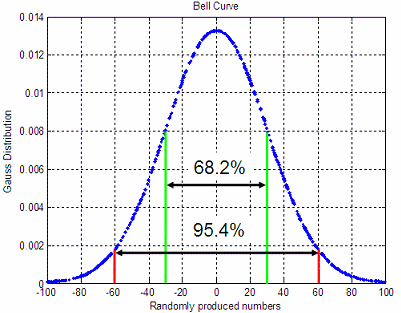
\includegraphics[width=0.35\columnwidth]{Graphics/gauss-distribution-002.png}~~~~~~ ~~~~
	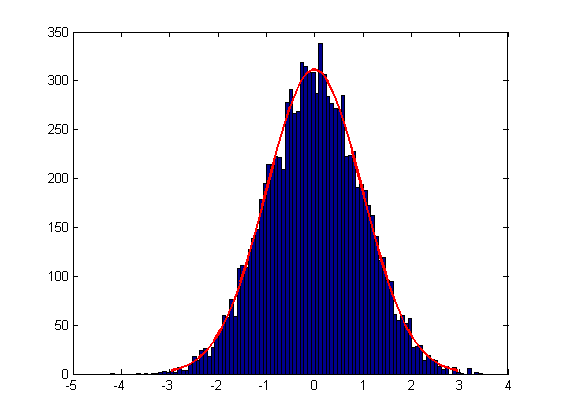
\includegraphics[width=0.35\columnwidth]{Graphics/O3lCB.png}
	\caption{(Left) Normal distribution $N(\mu, \sigma)$ with $\mu=0$ and $\sigma=30$. (Right) How do you determine the density? You have to collect data! The figure shows a ``fit'' of a normal distribution to data.}
\end{figure*}

\textbf{Def.}  $(\Omega, \mathscr{F}, P)$ is called a \ul{probability space}.
\begin{itemize}
\item $\Omega$ is the sample space. Think of it as the domain of a random variable $X: \Omega \to \real$ or random vector $X: \Omega \to \real^m$.
\item $A \subset \Omega$ is an event.
\item $\mathscr{F}$ is the collection of allowed events\footnote{Though it is too deep for ROB 501, there are subsets of the reals, for example, that are so complicated one cannot define a reasonable notion of probability that agrees with how we would want to define the probability of an interval, such as $[a, b]$.}. It must at least contain $\emptyset$ and $\Omega$. It is closed w.r.t. countable unions and intersections, and set complement.
    \item $P:\mathscr{F} \to [0, 1]$ is a probability measure. It has to satisfy a few basic operations
    \begin{itemize}
    \item $P(\emptyset)=0$ and $P(\Omega)=1$.
    \item For each $A \in \mathscr{F}$, $0 \le P(A) \le 1$
    \item If the sets $A_1, A_2, \ldots $ are disjoint (i.e., $A_i \cap A_j = \emptyset$ for $i \neq j$), then
    $$P\big(\bigcup_{i=1}^{\infty}A_i\big) = \sum_{i=1}^{\infty} P(A_i) $$
    \end{itemize}
\item Example event $A:=\{ \omega \in \Omega ~ |~ |\omega-\mu |\le \sigma \} \Rightarrow P(A)=0.682$
\end{itemize}

\newpage

    \section{Random Variables}

 \textbf{Def.}    $X: \Omega \rightarrow R$ is a \ul{random variable} if $\forall ~x \in \real$, the set
 $\{\omega \in \Omega~| X(\omega) \le x\} \in \mathscr{F} $. This just means that such sets can be assigned probabilities.

 \textbf{Remarks:} \begin{itemize}
 \item Shorthand notation $\{ X \le x\}:=\{\omega \in \Omega~| X(\omega) \le x\}$
 \item Because $\mathscr{F}$ is closed under set complements, (countable) unions, and (countable) intersections, we can also assign probabilities to

     \begin{itemize}
     \item[a)] $\{ X > x\}=\sim \{ X \le x\} = \{ X \le x\}^{C}$
     \item[b)] $\{ x < X \le y\}=\{ X \le y\} \bigcap \{ X > x\}$
     \end{itemize}


 \end{itemize}


 \textbf{Def.}   $X: \Omega \rightarrow \real$ is a \ul{continuous random variable} if there exists a \ul{density} $f:\real^p \to [0, \infty)$ such that,
 $$\forall~x\in \real,~~P\big(\{ X \le x\} \big)= \int_{-\infty}^{x} f(\bar{x}) d\bar{x}~~~(\bar{x}~~\text{dummy variable in the integral})$$



  \textbf{Remarks:}
  \begin{itemize}
 \item $\int_{a}^{b} f(x) dx=P\big( a < X \le b \big)=P\big( a \le X \le b \big)  $ \medskip \newline
 \hspace*{2cm}~$=P\big(\{\omega \in \Omega~|~ X(\omega) \in [a, b]\} \big)$

     \item mean: $\mu:=\E \{ X\}:= \int_{-\infty}^{\infty} x f(x) dx$

     \item Variance: $\sigma^2:=\E \{ (X-\mu)^2)\}:= \int_{-\infty}^{\infty} (x-\mu)^2f(x) dx$

     \item Standard Deviation $\sigma :=\sqrt{\sigma^2}$ (Std. Dev.)
     \end{itemize}

     \newpage

    \section{Random Vectors}
        \noindent
        \textbf{Def.} Let $(\Omega, \mathscr{F}, P)$ be a probability space. A function $X: \Omega \rightarrow \real^p$ is called a \ul{random vector} if each component of $X=\left[ \begin{array}{ccc}
        X_1\\X_2\\\vdots\\X_p\end{array} \right]$ is a random variable, that is, $\forall~ 1 \le i \le p$, $X_i: \Omega \rightarrow \real$   is a random variable.\\

        \setlength{\parskip}{.4in}

        \noindent
        \textbf{Consequence:} $\forall x \in \real^p $, the set $\{\omega \in \Omega \mid X(\omega) \le x\} \in \mathscr{F}$ (i.e., it is an allowed event), where the inequality is understood pointwise, that is,
        $$\{\omega \in \Omega \mid X(\omega) \le x \}:= \{\omega \in \Omega \mid \begin{bmatrix}X_1(\omega) \\X_2(\omega) \\ \vdots \\ X_p(\omega) \end{bmatrix} \le \begin{bmatrix} x_1 \\x_2 \\ \vdots \\ x_p \end{bmatrix} \} = \bigcap\limits^p_{i=1} \{\omega \in \Omega \mid X_i(\omega) \le x_i\}$$

         \textbf{Def.}   $X: \Omega \rightarrow \real^p$ is a \ul{continuous random vector} if there exists a \ul{density} $f:\real^p \to [0, \infty)$ such that,
 $$\forall~x\in \real^P,~~P\big(\{ X \le x\} \big)= \int_{-\infty}^{x_p} ... \int_{-\infty}^{x_2} \int_{-\infty}^{x_1}f_X(\bar{x}_1,\bar{x}_2...\bar{x}_p) d \bar{x}_1 d \bar{x}_2 ... d \bar{x}_p$$

 \newpage

\section{Moments}

\textbf{Def.} Suppose $g: \real^p \rightarrow R$
        $$E\{g(X)\}=\int_{\real^p}g(x)f_X(x)dx=\int_{-\infty}^{\infty}...\int_{-\infty}^{\infty}g(x_1,...,x_p)f_X(x_1,...,x_p)dx_1...dx_p$$

        \noindent
        \textbf{Mean or Expected Value}$$\mu=E\{X\}=E\{\left[ \begin{array}{ccc}X_1\\\vdots\\X_p\end{array} \right]\}=\left[ \begin{array}{ccc}\E\{X_1\}\\\vdots\\ \E\{X_p\}\end{array} \right]=
        \left[ \begin{array}{ccc}\mu_1\\\vdots\\\mu_p \end{array} \right]$$

        \noindent
        \textbf{Covariance Matrices}$$\Sigma:={\rm cov}(X)={\rm cov}(X,X)=E\{(X-\mu)(X-\mu)^T\}$$
        where
        $$(X-\mu) \mbox{ is }p\times 1 \mbox{, } (X-\mu)^T \mbox{ is }1\times p\mbox{, } (X-\mu)(X-\mu)^T \mbox{ is }p\times p$$

        \noindent
        \textbf{Exercise} cov(X) is positive semidefinite \\ \\

\newpage

   \section{Marginal Densities, Independence, and Correlatation}
        Suppose the random vector $X: \Omega \rightarrow \real^p$ is partitioned into two components $X_1 : \Omega \rightarrow R^n$ and $X_2:\Omega \rightarrow R^m $, with $p=n+m$, so that,
        $$ X = \left[ \begin{array}{cc} X_1 \\
                                               X_2 \end{array} \right]$$

\textbf{Notation:} We denote the density of $X$ by

$$f_X(x)=f_{\small \left[ \begin{array}{cc} X_1 \\
                                               X_2 \end{array} \right]}(x_1,x_2)=f_{X_1 X_2}(x_1,x_2) $$

and it is called the \ul{joint density} of $X_1$ and $X_2$. As before, we can define the mean and covariance.

 \begin{itemize}

 \item Mean is $\mu=
        \left[ \begin{array}{ccc}\mu_1\\ \mu_2 \end{array} \right]= \E\{X\}=E\{\left[ \begin{array}{ccc}X_1\\ X_2\end{array} \right]\}=\left[ \begin{array}{ccc}\E \{X_1\}\\ \E\{X_2\}\end{array} \right]$

 \item Covariance is \begin{align*} \Sigma =    \left[ \begin{array}{cc}\Sigma_{11} & \Sigma_{12}\\ \Sigma_{21} & \Sigma_{22}\end{array} \right] &= \E\{\left[ \begin{array}{c}X_1-\mu_1\\ X_2-\mu_2\end{array} \right] \left[ \begin{array}{c}X_1-\mu_1\\ X_2-\mu_2\end{array} \right]^\top\}  \\
     &= \E\{\left[ \begin{array}{c}X_1-\mu_1\\ X_2-\mu_2\end{array} \right] \left[ (X_1-\mu_1)^\top~~~ (X_2-\mu_2)^\top  \right] \} \\
     &= \E\{\left[ \begin{array}{cc}(X_1-\mu_1)(X_1-\mu_1)^\top &(X_1-\mu_1)(X_2-\mu_2)^\top \\
     (X_1-\mu_1)(X_2-\mu_2)^\top &(X_2-\mu_1)(X_2-\mu_2)^\top
     \end{array} \right]
     \end{align*}
 \end{itemize}
 where $\Sigma_{12}=\Sigma_{21}^\top = cov(X_1,X_2)=\E\{ (X_1-\mu_1)(X_2-\mu_2)^\top  \}$ is also called the \ul{correlation} of $X_1$ and $X_2$.



\newpage


If $X = \left[ \begin{array}{cc} X_1 \\
                                               X_2 \end{array} \right] :\Omega \to \real^{n+p}$ is a continuous random vector, then its components
                                               $$X_1:\Omega \to \real^n~~\text{and}~~X_2: \Omega \to \real^m$$ are also continuous random vectors and have densities, $f_{X_1}(x_1)$ and $f_{X_2}(x_2)$. These densities are given a special name.


 \textbf{Def.} $f_{X_1}(x_1)$ and $f_{X_2}(x_2)$  are called the \ul{marginal densities} of $X_1$ and $X_2$.

 \textbf{Fact: In general the marginal densities are a nightmare to compute.}  \begin{align*} f_{X_1}(x_1) &= \int_{-\infty}^{\infty} f_{X_1 X_2}(x_1, x_2) d x_2  \medskip \\
 &: =\int_{-\infty}^{\infty} \cdots \int_{-\infty}^{\infty} f_{X_1X_2}\big( \underbrace{ \bar{x}_1, \ldots, \bar{x}_n }_{x_1}, \underbrace{ \bar{x}_{n+1} , \cdots, \bar{x}_{n+m}}_{x_2} \big) \underbrace{d\bar{x}_{n+1} \cdots d\bar{x}_{n+m}}_{dx_2}\\
 \\
 f_{X_2}(x_2) &= \int_{-\infty}^{\infty} f_{X_1 X_2}(x_1, x_2) d x_1  \medskip \\
 &: =\int_{-\infty}^{\infty} \cdots \int_{-\infty}^{\infty} f_{X_1X_2}\big( \underbrace{ \bar{x}_1, \ldots, \bar{x}_n }_{x_1}, \underbrace{ \bar{x}_{n+1} , \cdots, \bar{x}_{n+m}}_{x_2} \big) \underbrace{d\bar{x}_{1} \cdots d\bar{x}_{n}}_{dx_1}\\
\end{align*}
For Normal Random Vectors, however, we can read them directly from the joint density! We will not be doing any iterated integrals.


        \noindent
        \textbf{Def. }$X_1$ and $X_2$ are \ul{independent random vectors} if their joint density factors
        $$f_X(x)=f_{X_1 X_2}(x_1,x_2)=f_{X_1}(x_1)f_{X_2}(x_2).$$

                \textbf{Def. }$X_1$ and $X_2$ are \ul{uncorrelated} if their ``cross covariance'' or ``correlation '' is zero
        $$cov(X_1,X_2) := \E \{ (X_1-\mu_1)(X_2-\mu_2)^\top \} = 0_{n \times m}$$

                        \textbf{Fact:} If $X_1$ and $X_2$ are independent, then they are also uncorrelated. \textbf{The converse is in general false.}

 \vspace*{2cm}

        \section{Conditioning}

        \noindent
        \textbf{Def.} For two events $A,B \in \mathscr{F}, P(B) > 0$
        $$P(A \mid B):=\frac{P(A\bigcap B)}{P(B)}$$
        is the \ul{conditional probability of $A$ given $B$}. \\

        \textbf{Remarks:}
        \begin{itemize}
        \item Suppose $P(A)$ is our current estimate of the probability that our robot is near a certain location and $B$ is a measurement of the robot's location, with confidence in the measurement being $P(B)$. The conditional probability of $A$ given $B$ occurred is how we ``fuse'' the two pieces of information
        $$P(A \mid B):=\frac{P(A\bigcap B)}{P(B)}$$

        \item
        $$B\subset A \mbox{, } P(A \mid B)=\frac{P(A\bigcap B)}{P(B)}=\frac{P(B)}{P(B)}=1$$
        \item
        $$A\subset B \mbox{, } P(A \mid B)=\frac{P(A\bigcap B)}{P(B)}=\frac{P(A)}{P(B)}\ge P(A)$$

        \end{itemize}

\newpage
Consider again our partitioned random vector $ X = \left[ \begin{array}{cc} X_1 \\
                                               X_2 \end{array} \right]$\\

          \textbf{Def.} The \ul{conditional density of $X_1$ given $X_2 = x_2$} is
          $$f_{X_1\mid X_2}(x_1 \mid x_2)=\frac{f_{X_1X_2}(x_1,x_2)}{f_{X_2}(x_2)}.$$
        Sometimes we simply write $f(x_1 \mid x_2)$\\

       \textbf{Remarks on Conditional Random Vectors:}
        \begin{itemize}

        \item \textbf{Very important:} $X_1$ given $X_2=x_2$ is (still) a random vector. It's density is $f_{X_1\mid X_2}(x_1 \mid x_2)$

        \item \textbf{Conditional Mean:} \begin{align*} \mu_{X_1 \mid X_2=x_2}&:=\E \{ X_1 \mid X_2=x_2\}  \\ \\ &:=\int_{-\infty}^{\infty} x_1 f_{X_1\mid X_2}(x_1 \mid x_2) dx_1
            \end{align*}
            $\mu_{X_1 \mid X_2=x_2}$ is a function of $x_2$. Think of it as a function of the value read by your sensor!

         \item  \textbf{Conditional Covariance:} \begin{align*} \Sigma_{X_1 \mid X_2=x_2} & := \E \{ (X_1 -\mu_{X_1 \mid X_2=x_2})(X_1 -\mu_{X_1 \mid X_2=x_2})^\top \mid X_2=x_2 \} \\ \\ &:=\int_{-\infty}^{\infty} (X_1 -\mu_{X_1 \mid X_2=x_2})(X_1 -\mu_{X_1 \mid X_2=x_2})^\top f_{X_1\mid X_2}(x_1 \mid x_2) dx_1
            \end{align*}
            $\Sigma_{X_1 \mid X_2=x_2}$ is a function of $x_2$. Think of it as a function of the value read by your sensor!

        \end{itemize}


\end{document}
